\documentclass[aspectratio=43,11pt]{beamer}

\usecolortheme{default}
\setbeamertemplate{navigation symbols}{}
\setbeamertemplate{footline}[frame number]
\usepackage[utf8]{inputenc}
\usepackage[T1]{fontenc}
\usepackage{amsmath,amssymb}
\usepackage{listings}
\usepackage{booktabs}
\usepackage{xcolor}
\definecolor{aggiemaroon}{RGB}{80,0,0}
\setbeamercolor{structure}{fg=aggiemaroon}
\setbeamercolor{frametitle}{fg=aggiemaroon}
\usepackage{tikz}
\usetikzlibrary{arrows.meta,positioning}

\lstset{
  basicstyle=\ttfamily\scriptsize,
  keywordstyle=\color{blue!70!black},
  commentstyle=\color{gray},
  frame=single,
  backgroundcolor=\color{gray!8},
  breaklines=true,
  language=R,
  showstringspaces=false
}

\title{Decision and Risk Analysis}
\subtitle{Lecture 11: \textbf{Evaluating Regression Models}}
\author{}
\date{\color{aggiemaroon}{DAEN 427 / ISEN 427 / ISEN 627 - Fall 2026\\
      \textbf{Alexander Abuabara}}}
\titlegraphic{\vfill 
\includegraphics[height=1.2cm]{TAMU_logo.png}}

\begin{document}

\begin{frame}
  \titlepage
\end{frame}

\begin{frame}{Roadmap}
  \tableofcontents
\end{frame}

%--------------------------------------------------------------
%\section{The Big Picture}

\begin{frame}{Why evaluate a model?}
  \begin{block}{Analogy}
    You would not eat a foraged mushroom or ride in a home-built car without checking it is safe. The same holds for models.
  \end{block}
  Three critical questions, for \emph{any} model (Bayesian or frequentist, simple or big):
  \begin{enumerate}
    \item \textbf{How fair} is the model?
    \item \textbf{How wrong} is the model?
    \item \textbf{How accurate} are the posterior predictive models?
  \end{enumerate}
  \vspace{0.4em}
  \textbf{Running example:} Capital Bikeshare (Washington, DC)
  \begin{align*}
    Y_i \mid \beta_0,\beta_1,\sigma &\overset{ind}{\sim} N(\mu_i,\sigma^2), \quad \mu_i=\beta_0+\beta_1X_i\\
    \beta_{0c}&\sim N(5000,1000^2),\;\; \beta_1\sim N(100,40^2),\;\; \sigma\sim\text{Exp}(0.0008)
  \end{align*}
  $Y$ = daily rides, $X$ = temperature (feels-like, $^\circ$F), $n=500$ days.
\end{frame}

%--------------------------------------------------------------
\section{Q1: Is the model fair?}

\begin{frame}{Question 1: Is the model fair?}
  Ask, \emph{every time}, even when the answer seems uneventful:
  \begin{itemize}
    \item How was the data collected?
    \item By whom, and for what purpose?
    \item How might the analysis or data collection impact individuals and society?
    \item What biases or power structures might be baked in?
  \end{itemize}
  \begin{alertblock}{Bikeshare check}
    Data come only from people who use the service. The model may better serve \emph{this} population at the exclusion of others. No perspective is neutral.
  \end{alertblock}
\end{frame}

\begin{frame}{Models are not always fair}
  \begin{itemize}
    \item \textbf{Hiring:} a r\'esum\'e-screening model trained on mostly male employees reinforced a preference for male applicants.
    \item \textbf{Facial recognition:} trained on unrepresentative images, so misidentification is more common for under-represented groups.
    \item \textbf{Risk classification:} a detention/release model that recommended detention in nearly all cases.
  \end{itemize}
  \vspace{0.5em}
  \begin{exampleblock}{Discussion}
    Which of the four fairness questions would have caught each of these problems earlier?
  \end{exampleblock}
\end{frame}

%--------------------------------------------------------------
\section{Q2: How wrong is the model?}

\begin{frame}{Question 2: How wrong is the model?}
  \begin{quote}
    ``All models are wrong, but some are useful.'' (George Box)
  \end{quote}
  The right question is not \emph{is} it wrong, but \emph{how} wrong. Check the three assumptions of
  $Y_i\mid\beta_0,\beta_1,\sigma\overset{ind}{\sim}N(\beta_0+\beta_1X_i,\sigma^2)$:
  \begin{enumerate}
    \item \textbf{Independence:} given $X$, cases are independent.
    \item \textbf{Linearity:} typical $Y$ is a linear function of $X$.
    \item \textbf{Normality and constant variance:} $Y$ varies normally around $\mu$ with the same $\sigma$ at every $X$.
  \end{enumerate}
  \begin{block}{Bikeshare}
    Ridership is correlated over time, but temperature explains much of that. Given $X$, independence is ``good enough to proceed.''
  \end{block}
\end{frame}

\begin{frame}{Posterior predictive check: the idea}
  If assumptions are reasonable, the posterior model should be able to \textbf{simulate data that looks like the observed data}.

  \medskip
  For each of the $N=20{,}000$ MCMC draws $\theta^{(j)}=(\beta_0^{(j)},\beta_1^{(j)},\sigma^{(j)})$ simulate $n=500$ outcomes:
  \[
    Y_i^{(j)}\sim N\!\left(\beta_0^{(j)}+\beta_1^{(j)}X_i,\;(\sigma^{(j)})^2\right)
  \]
  \[
    \begin{bmatrix}\theta^{(1)}\\ \vdots\\ \theta^{(N)}\end{bmatrix}
    \longrightarrow
    \begin{bmatrix}
      Y_1^{(1)}&\cdots&Y_{500}^{(1)}\\
      \vdots&&\vdots\\
      Y_1^{(N)}&\cdots&Y_{500}^{(N)}
    \end{bmatrix}
  \]
  \textbf{Rows} = simulated datasets (used here). \textbf{Columns} = posterior predictive model for one day (used later).
\end{frame}

\begin{frame}[fragile]{Posterior predictive check in R}
\begin{lstlisting}
library(bayesrules); library(rstanarm); library(bayesplot)

# bike_model <- stan_glm(rides ~ temp_feel, data = bikes,
#   family = gaussian,
#   prior_intercept = normal(5000, 1000),
#   prior = normal(100, 40),
#   prior_aux = exponential(0.0008),
#   chains = 4, iter = 5000*2, seed = 84735)

# Compare 50 of the 20,000 simulated datasets to the data
pp_check(bike_model, nreps = 50) + xlab("rides")
\end{lstlisting}
  \begin{itemize}
    \item \textbf{Dark curve} $y$: the observed data. \textbf{Light curves} $y_{rep}$: simulated datasets.
    \item \textbf{Bikes result:} center and range are captured, but most simulations miss the \textbf{bimodality}. Not a bad model, just one that could be \emph{less wrong}.
  \end{itemize}
\end{frame}

\begin{frame}{Reading a \texttt{pp\_check()}}
  \begin{columns}[T]
    \begin{column}{0.48\textwidth}
      \textbf{Good fit}
      \begin{itemize}
        \item Light curves wrap tightly around the dark curve
        \item Similar center, spread, and shape
      \end{itemize}
    \end{column}
    \begin{column}{0.48\textwidth}
      \textbf{Poor fit}
      \begin{itemize}
        \item Dark curve skewed, light curves symmetric
        \item Simulated $Y$ has wrong center or too much/little variability
        \item Missing modes, heavy tails, impossible values (e.g., negative counts)
      \end{itemize}
    \end{column}
  \end{columns}
  \vspace{0.6em}
  \begin{exampleblock}{Quick intuition}
    If you asked the model to ``write'' 50 fake datasets and a detective could instantly pick out the real one, the model is missing something.
  \end{exampleblock}
\end{frame}

\begin{frame}{Dealing with wrong models}
  \textbf{Assumption 1 fails} (dependent data)
  \begin{itemize}
    \item Repeated measures on the same subject (e.g., 3 memory tests per adult) $\Rightarrow$ \textbf{hierarchical models} (Unit 4, revisited at the end).
    \item Time/space dependence $\Rightarrow$ time series, spatial, spatiotemporal models.
  \end{itemize}
  \textbf{Assumptions 2 and 3 fail} (nonlinear, non-constant variance)
  \begin{itemize}
    \item \textbf{Different data structure:} Poisson, Negative Binomial, Binomial (Ch.\ 12--13).
    \item \textbf{Transform:} $g(Y)$, $h(X)$, or both, e.g.\ $\log(Y)$, $\sqrt X$, $X^2$.
  \end{itemize}
  \[
    \log(Y_i)\mid\beta_0,\beta_1,\sigma\overset{ind}{\sim}N(\beta_0+\beta_1X_i,\sigma^2)
  \]
  \textbf{Example:} $Y$ is right-skewed and its spread grows with $X$. After $\log(Y)$, the relationship is linear, the spread is constant, and the \texttt{pp\_check()} looks right.
\end{frame}

%--------------------------------------------------------------
\section{Q3: How accurate are the predictions?}

\begin{frame}{Question 3: How accurate are the posterior predictions?}
  A good model \textbf{generalizes} beyond the data used to build it. Three tools, from simplest to most technical:
  \begin{enumerate}
    \item Posterior predictive summaries (MAE, scaled MAE, within-50/95)
    \item Cross-validation (honest, out-of-sample versions of the same summaries)
    \item Expected log-predictive density (ELPD) for comparing models
  \end{enumerate}
\end{frame}

\begin{frame}[fragile]{One case: October 22, 2012}
  Temperature $=75^\circ$F, observed $Y=6228$ rides.
\begin{lstlisting}
predict_75 <- bike_model_df %>%
  mutate(mu = `(Intercept)` + temp_feel*75,
         y_new = rnorm(20000, mean = mu, sd = sigma))
\end{lstlisting}
  \begin{center}
  \begin{tabular}{lr}
    \toprule
    Posterior predictive mean $Y'$ & 3967\\
    Prediction error $Y-Y'$ & 2261\\
    Posterior sd & 1280\\
    Scaled error $(Y-Y')/\text{sd}$ & 1.767\\
    50\% interval & (3096, 4831) $\to$ \textbf{outside}\\
    95\% interval & (1500, 6482) $\to$ \textbf{inside}\\
    \bottomrule
  \end{tabular}
  \end{center}
  The model under-predicted, but the outcome was still within the realm of possibility.
\end{frame}

\begin{frame}{Why scale the error?}
  Two models both predict $Y'=3967$ and observe $Y=6228$ (error $=2261$ for both).
  \begin{center}
  \begin{tabular}{lrr}
    \toprule
     & Our model & Alternative\\
    \midrule
    Posterior sd & 1280 & 500\\
    Absolute error & 2261 & 2261\\
    Scaled error & \textbf{1.77} & \textbf{4.5}\\
    \bottomrule
  \end{tabular}
  \end{center}
  \begin{alertblock}{Takeaway}
    The same absolute error is far more damning when the model claimed to be confident. Scaling by the posterior sd accounts for the model's \emph{own} stated uncertainty. As a rule of thumb, $|{\rm scaled\ error}|>2$ or $3$ signals a poor prediction (for roughly symmetric posteriors).
  \end{alertblock}
\end{frame}

\begin{frame}{Posterior predictive summaries (all $n$ cases)}
  Each $Y_i$ has a posterior predictive mean $Y_i'$ and sd$_i$.
  \begin{itemize}
    \item \textbf{MAE} (median absolute error):
      $\;\text{median}\,|Y_i-Y_i'|$
    \item \textbf{Scaled MAE:}
      $\;\text{median}\,\dfrac{|Y_i-Y_i'|}{\text{sd}_i}$
    \item \textbf{within\_50 / within\_95:} proportion of observed $Y_i$ inside their 50\% / 95\% posterior prediction intervals.
  \end{itemize}
  \vspace{0.3em}
  \textbf{Calibration check:} within\_50 should be near 0.50 and within\_95 near 0.95.

  \medskip
  \texttt{stable = TRUE} switches to the median and median absolute deviation, which is useful for skewed posteriors.
\end{frame}

\begin{frame}[fragile]{Bikeshare: summaries on the training data}
\begin{lstlisting}
set.seed(84735)
predictions <- posterior_predict(bike_model, newdata = bikes)
dim(predictions)   # 20000 x 500
ppc_intervals(bikes$rides, yrep = predictions,
              x = bikes$temp_feel, prob = 0.5, prob_outer = 0.95)

prediction_summary(bike_model, data = bikes)
\end{lstlisting}
  \begin{center}
  \begin{tabular}{rrrr}
    \toprule
    mae & mae\_scaled & within\_50 & within\_95\\
    \midrule
    989.7 & 0.7712 & 0.438 & 0.968\\
    \bottomrule
  \end{tabular}
  \end{center}
  Typically, ridership is about 990 rides (0.77 sd) from its prediction. 43.8\% of days fall in their 50\% interval and 96.8\% in their 95\% interval. Is 990 good enough? \textbf{It depends on context} (ask Capital Bikeshare).
\end{frame}

%--------------------------------------------------------------
\begin{frame}{The problem: testing on the data you trained on}
  \begin{block}{The anchov-lada analogy}
    You build every taco recipe around Reem, who loves anchovies. Her approval does not mean the general public will like it.
  \end{block}
  A model is optimized to the data it was built on, so evaluating accuracy on that \emph{same} data is \textbf{overly optimistic}.

  \medskip
  \textbf{Idea:} split the existing data into roles.
  \begin{itemize}
    \item \textbf{Train:} build the model on, say, 90\% (450 days).
    \item \textbf{Test:} predict the held-out 10\% (50 days) and compute MAE, etc.
  \end{itemize}
  One split is \textbf{unstable}: a different random split may paint a different picture.
\end{frame}

\begin{frame}{$k$-fold cross-validation}
  \begin{enumerate}
    \item \textbf{Create folds:} split data into $k$ non-overlapping folds of roughly equal size.
    \item \textbf{Train and test:} train on $k-1$ folds, test on the remaining one, record MAE etc.
    \item \textbf{Repeat} $k-1$ more times, each time holding out a different fold.
    \item \textbf{Average} the $k$ measures into one cross-validation estimate.
  \end{enumerate}
  \vspace{0.4em}
  \begin{center}
  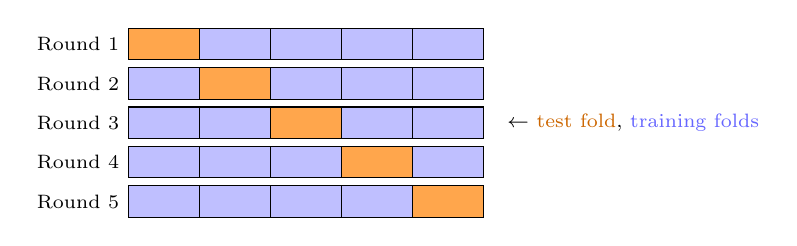
\begin{tikzpicture}[x=0.9cm,y=0.5cm,font=\scriptsize]
    \foreach \r in {1,2,3,4,5}{
      \foreach \c in {1,...,5}{
        \pgfmathparse{\r==\c ? "orange!70" : "blue!25"}
        \edef\col{\pgfmathresult}
        \draw[fill=\col] (\c,-\r) rectangle ++(1,0.8);
      }
      \node[anchor=east] at (1,-\r+0.4) {Round \r};
    }
    \node[anchor=west] at (6.2,-3+0.4) {$\leftarrow$ \textcolor{orange!80!black}{test fold}, \textcolor{blue!60}{training folds}};
  \end{tikzpicture}
  \end{center}
  \textbf{Choosing $k$ (Goldilocks):} $k=2$ trains on too little data (pessimistic). $k=n$ is leave-one-out (LOO): needs $n$ models (slow). $k=10$ is a common compromise.
\end{frame}

\begin{frame}[fragile]{Cross-validation in R and results}
\begin{lstlisting}
set.seed(84735)
cv_procedure <- prediction_summary_cv(
  model = bike_model, data = bikes, k = 10)
cv_procedure$folds   # metrics per fold
cv_procedure$cv      # averaged estimate
\end{lstlisting}
  \begin{center}
  \begin{tabular}{lrrrr}
    \toprule
     & mae & mae\_scaled & within\_50 & within\_95\\
    \midrule
    In-sample & 989.7 & 0.7712 & 0.438 & 0.968\\
    10-fold CV & 1029 & 0.8015 & 0.420 & 0.968\\
    \bottomrule
  \end{tabular}
  \end{center}
  Per-fold MAE ranged from about 787 to 1271. To predict tomorrow's ridership, expect to be off by about \textbf{1029 rides}, not 990. In-sample summaries gave a rosier picture.
\end{frame}

%--------------------------------------------------------------
\begin{frame}{Expected log-predictive density (ELPD)}
  The posterior predictive pdf for a new day:
  \[
    f(y'\mid\vec y)=\int f(y'\mid\theta)\,f(\theta\mid\vec y)\,d\theta
  \]
  The higher $f(y_{\text{new}}\mid\vec y)$ (equivalently its log) at the value that actually occurs, the better the prediction.
  \begin{block}{ELPD}
    The average of $\log f(y_{\text{new}}\mid\vec y)$ over possible new data points. \textbf{Higher is better.}
  \end{block}
\end{frame}

\begin{frame}[fragile]{Computing and using ELPD}
\begin{lstlisting}
model_elpd <- loo(bike_model)   # leave-one-out CV
model_elpd$estimates
#          Estimate      SE
# elpd_loo  -4289.0 13.1186
# p_loo         2.5  0.1638
# looic      8578.1 26.2371
\end{lstlisting}
  \begin{itemize}
    \item ELPD $=-4289$ is hard to interpret alone; its scale changes from analysis to analysis.
    \item Its power is in \textbf{comparing models fit to the same data}:
  \end{itemize}
\begin{lstlisting}
loo_compare(loo(model_1), loo(model_2))  # larger elpd wins
\end{lstlisting}
\end{frame}

\begin{frame}{Improving posterior predictive accuracy}
  \begin{enumerate}
    \item \textbf{Collect more data.} It cannot strengthen a weak $Y$--$X$ relationship, but it improves our understanding of it.
    \item \textbf{Use different or more predictors.} Maybe humidity beats temperature, or use both (Chapter 11). There are limits to this strategy.
  \end{enumerate}

  \begin{alertblock}{Two different questions}
    \textbf{How good is the MCMC simulation?} (trace plots, $\hat R$, effective sample size)\\
    \textbf{How good is the model?} (fair, not too wrong, accurate)

    You can approximate a good model badly, or approximate a bad model well.
  \end{alertblock}
\end{frame}

\begin{frame}{Summary: the evaluation checklist}
  \begin{center}
  \small
  \begin{tabular}{p{2.2cm}p{4.2cm}p{3.3cm}}
    \toprule
    \textbf{Question} & \textbf{Tool} & \textbf{Look for}\\
    \midrule
    Fair? & Context, ethics review & No harmful bias, appropriate use\\[0.4em]
    Wrong? & \texttt{pp\_check()} & Simulated data resemble observed data\\[0.4em]
    Accurate? & \texttt{prediction\_summary()}, \texttt{prediction\_summary\_cv()}, \texttt{loo()} & Small MAE, calibrated within\_50/95, higher ELPD\\
    \bottomrule
  \end{tabular}
  \end{center}
  Always prefer \textbf{cross-validated} metrics when judging how well a model will predict new data.
\end{frame}

%--------------------------------------------------------------
\section{Normal Hierarchical Models}

\begin{frame}{Why a hierarchical model?}
  \textbf{Grouped data:} observations within groups $j=1,\dots,J$ are correlated (violating independence), e.g.\ several songs per artist, several tests per student.
  \vspace{.5cm}
  \begin{columns}[T]
    \begin{column}{0.32\textwidth}
      \textbf{Complete pooling}\\
      Ignore groups; one mean $\mu$ for everyone.\\
      \emph{Ignores group differences.}
    \end{column}
    \begin{column}{0.32\textwidth}
      \textbf{No pooling}\\
      Separate mean $\mu_j$ per group, estimated in isolation.\\
      \emph{Noisy for small groups; cannot generalize.}
    \end{column}
    \begin{column}{0.32\textwidth}
      \textbf{Partial pooling}\\
      Group means share a common distribution.\\
      \emph{Borrows strength across groups.}
    \end{column}
  \end{columns}
\end{frame}

\begin{frame}{The Normal hierarchical model (no predictors)}
  \begin{align*}
    Y_{ij}\mid\mu_j,\sigma_y &\sim N(\mu_j,\sigma_y^2) &&\text{within-group (layer 1)}\\
    \mu_j\mid\mu,\sigma_\mu &\sim N(\mu,\sigma_\mu^2) &&\text{between-group (layer 2)}\\
    \mu,\;\sigma_y,\;\sigma_\mu &\sim \text{priors} &&\text{global parameters (layer 3)}
  \end{align*}
  \begin{itemize}
    \item $\mu$: global average. $\mu_j$: group-specific average.
    \item $\sigma_y$: \textbf{within-group} variability. $\sigma_\mu$: \textbf{between-group} variability.
  \end{itemize}
  \begin{block}{Intraclass correlation}
    The fraction of total variance due to group differences:
    \[
      \text{ICC}=\frac{\sigma_\mu^2}{\sigma_\mu^2+\sigma_y^2}
    \]
  \end{block}
\end{frame}

\begin{frame}{Evaluating a hierarchical model: the same three questions}
  \begin{enumerate}
    \item \textbf{Fair?} Are all groups represented? Are small or under-represented groups hurt by shrinkage toward the overall mean?
    \item \textbf{Wrong?} Use \texttt{pp\_check()}: simulate $Y_{ij}$ through \emph{both} layers and compare with the data. Also check whether the Normal assumption for the $\mu_j$ is plausible (look at group-level estimates).
    \item \textbf{Accurate?} Posterior predictive summaries, \textbf{cross-validation} (done carefully), and ELPD for comparing pooling strategies.
  \end{enumerate}
\end{frame}

\begin{frame}[fragile]{Step 1: Is it wrong? Posterior predictive check}
\begin{lstlisting}
# Hierarchical model with only a group-level intercept
hier_model <- stan_glmer(
  y ~ (1 | group), data = dat, family = gaussian,
  chains = 4, iter = 5000*2, seed = 84735)

pp_check(hier_model, nreps = 50)
\end{lstlisting}
  \begin{itemize}
    \item Does the overall shape of $y_{rep}$ match $y$?
    \item Also check by group: if a group's data consistently sits outside its simulations, the common $N(\mu,\sigma_\mu^2)$ for group means (or constant $\sigma_y$) may be wrong.
    \item Compare $\sigma_y$ vs.\ $\sigma_\mu$ to see where the variability lives (ICC).
  \end{itemize}
\end{frame}

\begin{frame}{Step 2: Accuracy: two kinds of predictions}
  \begin{columns}[T]
    \begin{column}{0.48\textwidth}
      \textbf{(a) A new case from an existing group $j$}
      \[
        Y_{\text{new},j}\mid\vec y\sim N(\mu_j,\sigma_y^2)
      \]
      using the posterior for \emph{that group's} $\mu_j$ (narrower, group-specific).
    \end{column}
    \begin{column}{0.48\textwidth}
      \textbf{(b) A case from a brand-new group}
      \[
        \mu_{\text{new}}\sim N(\mu,\sigma_\mu^2),\;\; Y\sim N(\mu_{\text{new}},\sigma_y^2)
      \]
      Uncertainty includes $\sigma_\mu$ (wider).
    \end{column}
  \end{columns}
  \vspace{0.5em}
  \textbf{Evaluate each scenario separately.} Predicting a new group is harder and is the more honest test of generalization.
\end{frame}

\begin{frame}[fragile]{Cross-validation for grouped data}
  Folds must respect the question you care about.
\begin{lstlisting}
# In-sample summaries (existing groups)
set.seed(84735)
prediction_summary(hier_model, data = dat)

# New groups: hold out whole groups at a time
prediction_summary_cv(model = hier_model, data = dat,
                      group = "group", k = 10)

# ELPD (LOO) to compare pooling strategies
loo_compare(loo(complete_pool), loo(no_pool), loo(hier_model))
\end{lstlisting}
  Compare complete, no, and partial pooling by cross-validated MAE and ELPD. Partial pooling typically wins when groups differ but have limited data each.
\end{frame}

\begin{frame}{Shrinkage and the bias--variance trade-off}
  The hierarchical estimate of a group mean is a weighted average:
  \[
    \hat\mu_j\approx \underbrace{w_j\,\bar y_j}_{\text{group data}}+\underbrace{(1-w_j)\,\hat\mu}_{\text{global mean}},
    \qquad
    w_j=\frac{n_j/\sigma_y^2}{n_j/\sigma_y^2+1/\sigma_\mu^2}
  \]
  \begin{itemize}
    \item Small $n_j$ or large $\sigma_y$: $w_j$ small, \textbf{more shrinkage} toward $\hat\mu$.
    \item Large $n_j$ or large $\sigma_\mu$: $w_j$ large, \textbf{less shrinkage}.
  \end{itemize}
  Shrinkage adds a little \textbf{bias} but reduces \textbf{variance}, which usually improves out-of-sample prediction.
\end{frame}

\begin{frame}{Worked example: three classrooms}
  Test scores; global mean $\hat\mu=75$, $\sigma_y=10$, $\sigma_\mu=5$.
  \begin{center}
  \begin{tabular}{lrrrr}
    \toprule
    Classroom & $n_j$ & $\bar y_j$ & $w_j$ & $\hat\mu_j$\\
    \midrule
    A & 4 & 90 & 0.50 & 82.5\\
    B & 25 & 90 & 0.86 & 87.9\\
    C & 100 & 90 & 0.96 & 89.4\\
    \bottomrule
  \end{tabular}
  \end{center}
  Same raw average (90), different shrinkage. Evidence for A is thin, so its estimate is pulled strongly toward 75; C barely moves.
  \begin{exampleblock}{Why it helps prediction}
    A small class that scored 90 by luck will likely score lower next time. The shrunken estimate anticipates this and gives better future predictions.
  \end{exampleblock}
\end{frame}

\begin{frame}{Hierarchical evaluation checklist}
  \begin{itemize}
    \item \textbf{Fair:} no group systematically disadvantaged by pooling or by who is in the data.
    \item \textbf{Wrong:} \texttt{pp\_check()} overall and by group; sanity-check normality of group effects and constant $\sigma_y$.
    \item \textbf{Accurate:}
      \begin{itemize}
        \item Separate summaries for \emph{existing-group} and \emph{new-group} prediction.
        \item Cross-validation that holds out observations or whole groups.
        \item ELPD (\texttt{loo}) to compare complete, no, and partial pooling.
      \end{itemize}
    \item \textbf{Remember:} separately check MCMC quality (R-hat, effective sample size). Hierarchical posteriors can be harder to sample.
  \end{itemize}
\end{frame}

%--------------------------------------------------------------
\section{Practice Questions}

\begin{frame}{Practice Questions (1/2)}
  \begin{enumerate}
    \item Name the three big questions for evaluating any model.
    \vspace{0.6em}
    \item In a \texttt{pp\_check()}, what does the dark curve represent, and what does each light curve represent?
    \vspace{0.6em}
    \item Model A and Model B both predict $Y'=50$ and observe $Y=60$. Model A has posterior sd $=2$; Model B has sd $=10$. Which model predicted better, and why?
    \vspace{0.6em}
    \item Your model's cross-validated MAE is larger than its in-sample MAE. Is that surprising? Why?
  \end{enumerate}
\end{frame}

\begin{frame}{Practice Questions (2/2)}
  \begin{enumerate}
    \setcounter{enumi}{4}
    \item A model has within\_95 $=0.70$. What does that suggest?
    \vspace{0.6em}
    \item Why is a single ELPD value hard to interpret, and what is it best used for?
    \vspace{0.6em}
    \item In 10-fold CV with $n=500$, how many models are trained and how many points are in each training set?
    \vspace{0.6em}
    \item In a Normal hierarchical model, a group has $n_j=3$ observations. Will its estimate be shrunk more or less than a group with $n_j=300$?
    \vspace{0.6em}
    \item When evaluating a hierarchical model, why evaluate ``new group'' prediction separately from ``existing group'' prediction?
  \end{enumerate}
\end{frame}

\begin{frame}{Quick Answers (1/2)}
  \begin{enumerate}
    \item \textbf{Fair? Wrong? Accurate?} (data/context/ethics; assumptions via posterior predictive check; predictive accuracy of the posterior predictive models).
    \item Dark curve: the observed data $y$. Each light curve: one dataset $y_{rep}$ simulated from the posterior model at one parameter draw.
    \item \textbf{Model B.} Absolute errors are equal (10), but scaled errors are $10/2=5$ for A and $10/10=1$ for B. Model A is overconfident: the observation is 5 sds from its prediction, while B's predictive model comfortably covers it.
    \item Not surprising. In-sample evaluation is optimistic because the model was fit to those same points; cross-validation gives a more honest estimate of error on new data.
  \end{enumerate}
\end{frame}

\begin{frame}{Quick Answers (2/2)}
  \begin{enumerate}
    \setcounter{enumi}{4}
    \item The 95\% prediction intervals are too narrow: only 70\% of observations fall inside, instead of about 95\%. The model is overconfident, so assumptions (e.g.\ variance or shape) may be wrong.
    \item The ELPD scale depends on the data and model, so no universal ``good'' value exists. Use it to \textbf{compare models} fit to the same data; higher is better.
    \item 10 models; each trained on $9/10\cdot 500=450$ points and tested on 50.
    \item \textbf{More} shrinkage toward the global mean, since little data about that group means the weight $w_j$ on its own sample mean is small.
    \item Predicting a new group also requires uncertainty about the group mean ($\sigma_\mu$), so it is harder and has wider intervals. Accuracy for existing groups can look good while generalization to new groups is poor.
  \end{enumerate}
\end{frame}

\end{document}